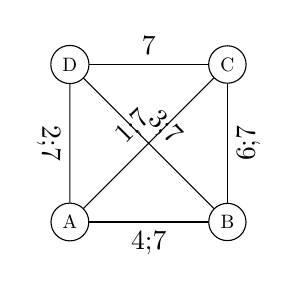
\begin{tikzpicture}[gv/.style={draw=black,circle,scale=0.7},scale=2]
\node[gv] (A) at (0,0) {A};
\node[gv] (B) at (1,0) {B};
\node[gv] (D) at (0,1) {D};
\node[gv] (C) at (1,1) {C};
\draw (A) to node[sloped,below] {4;7} (B) to node[sloped,below] {6;7} (C) to node[sloped,above] {7} (D);
\draw (B) to node[sloped,above] {3;7} (D) to node[sloped,below] {2;7} (A) to node[sloped,above] {1;7} (C);
\end{tikzpicture}